\chapter{Evaluation}
This chapter compares the performance of my compiler with three existing alternatives for running code on the web: Compiling C to WebAssembly with Clang/LLVM, compiling Grain (a functional language based on OCaml that compiles to WebAssembly), and translating OCaml programs to JavaScript with the Js\_of\_ocaml tool.
I also measure the impact of the optimisations implemented in my compiler. Performance is based on three metrics: 

\begin{itemize}
\item \textbf{Execution time}: This is measured by a JavaScript program, run using Node.js, for each of the alternatives. Timing information is obtained from the \verb|performance| interface, which has up to microsecond precision and is not affected by system time changes, so is guaranteed to be monotonic \cite{timing}. This is sampled over 20 runs of the program and the mean and 95\% confidence interval are recorded. 

\item \textbf{Heap usage}: The heap memory used is also collected by these scripts. Without garbage collection, my runtime allocates memory linearly so a call to allocate 0 bytes returns the total memory used. For the garbage-collected allocator, I created a separate version which tracks the peak memory allocated, updating this on each allocation. 

The Grain runtime's development build outputs similar memory tracing statistics, including the amount of heap memory used. 
The overhead of tracing is significant so this is done separately to collecting timing information. For C, where parts of \verb|stdlib| are included in the WebAssembly output for memory allocation, \verb|sbrk(0)| returns the size of the WebAssembly linear memory used. 
Lastly, for programs translated to JavaScript, the benchmarking script is run with the \verb|--expose-gc| option. This allows calling the garbage collector before the program is executed, and approximating the memory used by calling \verb|process.memoryUsage().heapUsed| before and after the program runs. This is an approximate value, so it is also averaged over 20 iterations.

\item \textbf{Output file size}: This is easily obtained from the file system.

\end{itemize}

\newpage
\section{Microbenchmarks}
I wrote a set of test programs, each aiming to represent a different programming style, to see how performance varied across applications. The programs were also parameterised so that comparisons could be made at different problem sizes. % Only a few instances of this are included in the data to keep the number of dimensions of comparison manageable, instead focusing more on other aspects. The microbenchmarks used were:
Where available, these programs were based on code from existing benchmarking libraries.

% TODO: Rename everywhere so I can use other names instead
\begin{itemize}
\item \verb|alltrees|: Constructs a list of all binary trees of a given size, which is very memory intensive. % and objects that exist for varying lifetimes.

\item \verb|arith|: Computes Euler's totient function for all integers from 1 to a given \verb|n|, involving a large amount of integer arithmetic. This was based on problem 34 of the 99 Problems in OCaml \cite{99-problems}, implementing Euler's totient function.

\item \verb|composition|: Constructs a function which is the composition of a list of simple functions and maps it over a list, making heavy use of higher-order functions.

\item \verb|funcrec| (functions, records): Compares three forms of parameterisation: Using functions defined at the top-level of a program, passing those functions as arguments, and passing those functions as fields of a record argument. This was based on an existing repository of OCaml benchmarks available on GitHub \cite{chris00}.

\item \verb|mergesort|: Implements mergesort, making heavy use of lists and pattern matching.

\item \verb|nbody|: Simulates the n-body problem, simulating the motion of planets for a number of time steps and making heavy use of floating-point arithmetic. This was adapted from the version in the Computer Language Benchmarks Game repository \cite{benchmark-game}.
\end{itemize}

%A couple other microbenchmarks were also used to demonstrate the worst-case behaviour some optimisations aim to avoid. These will be described later when the data for those optimisations is presented. 


\section{Comparison against alternatives}
Although most of the runtime for my compiler is written in WebAssembly, the garbage-collected memory allocator is written in JavaScript due to its complexity and wanting to make several improvements to it. Therefore, the performance of my compiler is indicated with and without garbage collection, to distinguish the overhead of calling between WebAssembly and JavaScript for each memory allocation. The data given is also for the optimised version of the compiler.

\subsection{Execution Time}

\begin{figure}[H]
\hspace{-0.7cm}
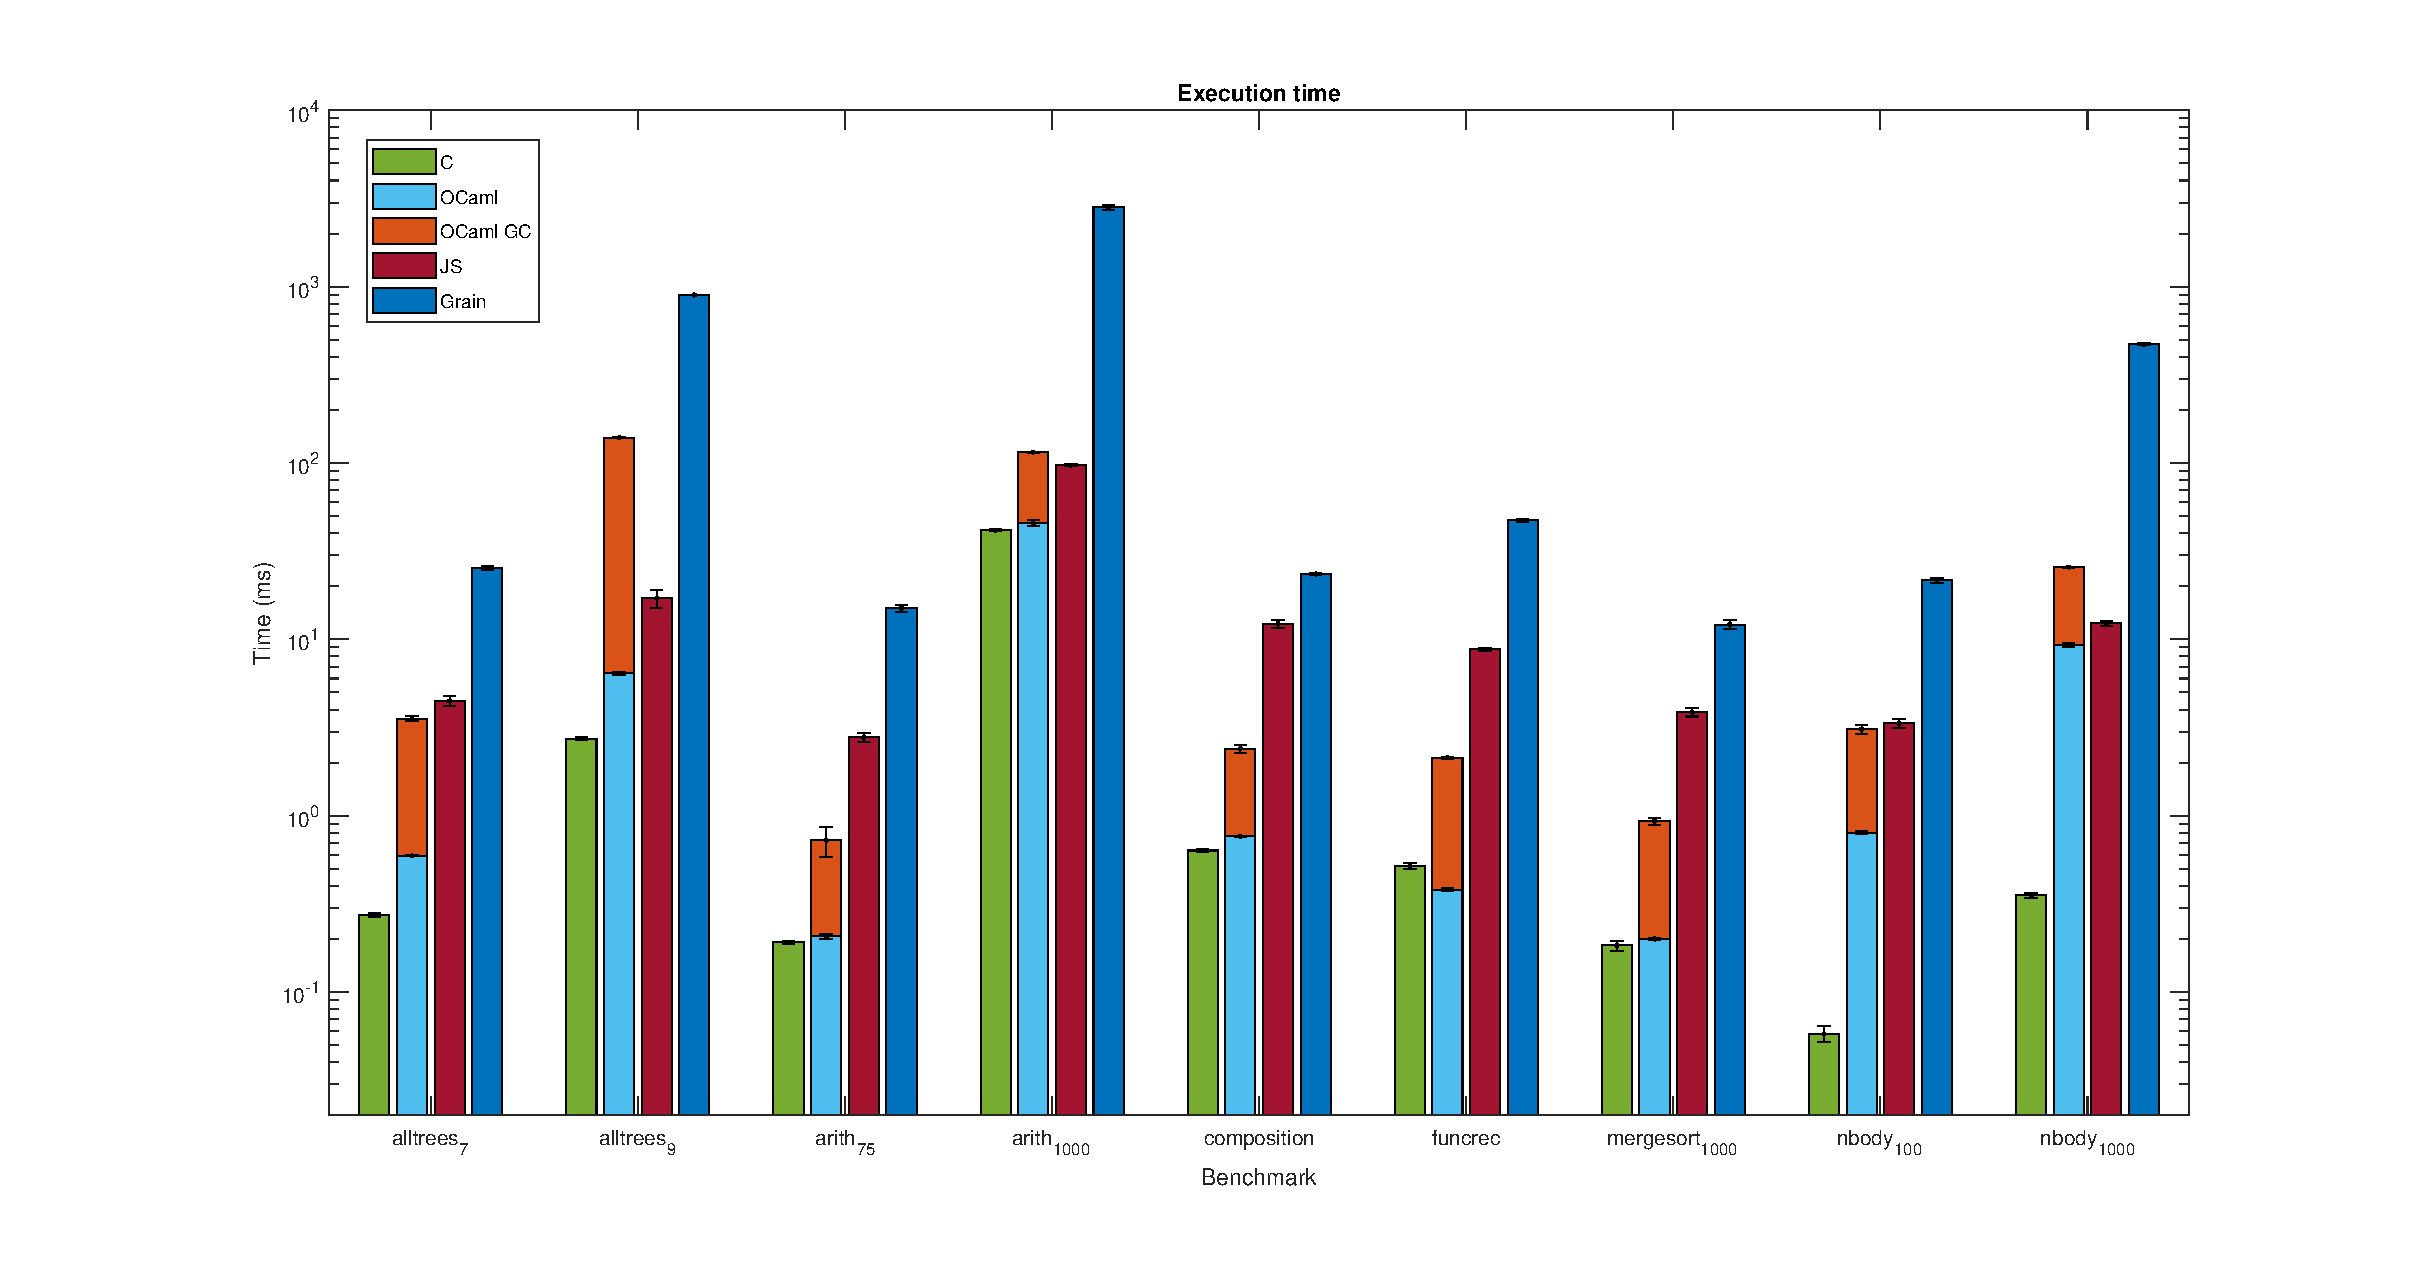
\includegraphics[scale=0.42]{figures/alternatives_timing}
\vspace{-0.5cm}
\caption{Execution times for each alternative}
 \label{fig:alt_timing} 
\end{figure}

First, we see that the execution speed can vary by a couple orders of magnitude between the least and most efficient method. Unsurprisingly, the programs translated to C by hand and compiled to WebAssembly are the fastest. At the opposite end, Grain is always significantly slower than the other methods. My compiler is always faster than the equivalent JavaScript when run without garbage collection, however the overhead of garbage collection results in the two being more balanced, as shown further in figure \ref{fig:js_oc_timing}.% performing better on some programs and worse on others. This is shown in more detail below:


\begin{figure}[H]
\hspace{-1.6cm}
\includegraphics[scale=0.52]{figures/js_ocaml_timing}
\vspace{-0.5cm}
\caption{Comparison between my compiler and Js\_of\_ocaml}
 \label{fig:js_oc_timing} 
\end{figure}

Without garbage collection, my compiler's output	executes between 0.33 and 20 times faster than the JavaScript program produced by  Js\_of\_ocaml. With garbage collection, execution time grows much faster with problem size and my compiler performs worse for programs making a large number of memory allocations.

%it still outperforms the JavaScript alternative in most cases, except for programs making a very large number of memory allocations such as \verb|alltrees| with a large problem size.


\subsection{Heap usage}

\begin{figure}[H]
\hspace{-1cm}
\includegraphics[scale=0.43]{figures/alternatives_heap}
\vspace{-0.5cm}
\caption{Heap usage for each alternative}
 \label{fig:alt_heap} 
\end{figure}

There are no bars for C for \verb|arith|, \verb|funcrec| and \verb|nbody|, as these did not require the heap to implement. 
% TODO: Should try to get some value for Grain Arith_1000, even if very few iterations
There is also no data for Grain for \verb|arith_1000| as the program did not appear to terminate with tracing enabled.
% was very slow without tracing (see figure \ref{fig:alt_timing}) and with tracing enabled did not terminate after 10 minutes.

Where the compiled C programs did use the heap, my garbage-collected runtime uses at worst 13\% more memory. My implementation also uses significantly less memory than both the JavaScript and Grain alternatives. In every test, % (ignoring the Grain result for \verb|arith_1000|), 
the garbage-collected runtime uses at most one third of the memory used by either the JavaScript or Grain version. 

The order of the bars for my compiler, with and without garbage collection, are reversed in three of the tests. These tests have fewer opportunities for garbage collection so it saves little memory, but the implementation consumes more memory due to the overhead of headers and trailers on allocated blocks. In the worst case, \verb|funcrec| has no opportunities for garbage collection and almost exclusively allocates small objects of 8 bytes. Since each header and trailer is 8 bytes, garbage collection triples the amount of memory used.



\subsection{Output File Size}

\begin{figure}[H]
\hspace{-1cm}
\includegraphics[scale=0.6]{figures/alternatives_size}
\vspace{-0.8cm}
\caption{Output size for each alternative}
 \label{fig:alt_size} 
\end{figure}

As expected, the JavaScript output tends to be largest as JavaScript is a text format rather than a binary format like WebAssembly. On average, it is 8 times larger than the output of my compiler with garbage collection enabled. Grain also produces much larger binary files, averaging about 3.5 times larger than my compiler's output. Inspecting the compiled output, there appears to be a few reasons for this. First, programs import a larger set of functions from Grain's runtime than used by my compiler, as Grain supports more types of numerical data, such as having both 32-bit and 64-bit integers. It also uses a reference counting garbage collector, which adds more overhead since updating a variable requires both incrementing the new value and decrementing the old value, whereas my garbage collector just overwrites the old value on the shadow stack. Lastly, it does not appear to optimise the WebAssembly produced, compared with my compiler which uses a register allocation algorithm to reduce the number of local variables declared, and peephole optimises trivially useless statements such as \verb|local.get i; drop|.

Compared with the output of compiling a C program, the sizes are similar except where parts of \verb|stdlib| have to be included for memory allocation, which makes those programs about 7KB larger. For comparison, my runtime without garbage collection is a 740B WebAssembly file, but the garbage collector is implemented in JavaScript, which when minified is a 4KB file.

Lastly, this demonstrates the overhead of garbage collection in terms of the extra bookkeeping operations added to maintain the shadow stack. On average, this adds about 30\% to the size of the output WebAssembly.

\section{Optimisations}

I first compare the impact of the IR and WebAssembly optimisations and their combined effect on performance. After that, I look at the impact of specific optimisations at the IR level by seeing how performance changes when one is removed, and the benefit of optimising pattern matching. Finally, I show the benefit of repeating the optimisation passes multiple times. %, as well as looking at how the phase ordering at the IR level impacts performance.  -- LEAVE THIS FOR IF SECTION TOO SHORT
Data is collected with garbage collection disabled. % to exclude the overhead it introduces.

\subsection{IR and WebAssembly optimisations}
\vspace{-0.4cm}
\begin{figure}[H]
\vspace{-0.05cm}
\hspace{-0.5cm}
\includegraphics[scale=0.45]{figures/opts_threeplots}
\vspace{-0.6cm}
\caption{Performance with IR and WebAssembly optimisations}
 \label{fig:opts} 
\end{figure}
The peephole optimisations done at the WebAssembly level have no impact on memory usage or execution time, but consistently reduce output size by about 10\%. The IR optimisations reduce execution time and heap usage by at least 30\% for all microbenchmarks, except \verb|nbody|. \verb|nbody| is the only program which does not improve in all metrics, and instead executes 3\% slower. It is an imperative style program, which may explain why the optimisations perform well on the other programs but not on it, since they are unable to optimise uses of mutable variables and \verb|nbody| has no recursion to optimise either. 
 For \verb|arith| and \verb|funcrec|, inlining or rewriting functions has completely removed the need to construct closures recursively, resulting in near zero heap usage. %The execution time of \verb|nbody| is the only case where optimisations decrease performance, but only by 3\%.  \verb|nbody| is an imperative style program, which may explain why the optimisations perform well on the other programs but not on it, since they are unable to optimise uses of mutable values and \verb|nbody| has no recursion to optimise.

\subsection{Impact of inlining, uncurrying and tail calls}
\vspace{-0.4cm}
\begin{figure}[H]
\hspace{-0.8cm}
\includegraphics[scale=0.45]{figures/specific_opts}
\vspace{-1cm}
\caption{Impact of individual optimisations}
 \label{fig:specific-opts} 
\end{figure}

Figure \ref{fig:specific-opts} shows the change when one optimisation is removed, so the magnitude of each bar can be viewed as the speed-up or size reduction an optimisation has, on top of the optimisations already present. First, inlining only increases file size in one case, \verb|funcrec|, and only by 5\%, so the optimisation is not causing significant code bloat. Instead, inlining reduces the size of the output in cases where it completely removes a function definition. Overall, it has a relatively small impact on performance, with the biggest change being a 15\% speed-up for \verb|funcrec|. This suggests that the heuristics used for inlining may be too conservative, and allowing inlining in more places could improve performance while still keeping code size reasonable. However, these are all relatively small benchmark programs, which could also be limiting how significant a change can be achieved by inlining. % suggesting that either the heuristics for inlining were too restrictive or that this set of microbenchmarks or other optimisations are not complex enough to see significant improvements from inlining.

% Getting too specific? Talk in higher-level general details?
Tail-call optimisation does not affect most of the programs, but improves the execution speed of \verb|funcrec| and the speed and file size for \verb|arith|. A more important factor, not shown by figure \ref{fig:specific-opts}, is that tail-call optimisation allows some programs to execute that would otherwise give an error: \\
\verb|let rec f x = if x = 0 then 0 else f (x-1)| \\
Despite this being a very simple function, without tail-call optimisation, calling \verb|f(30000)| exceeds the maximum call stack size and the program fails. With tail-call optimisation, the function no longer makes recursive calls so can handle any input size.

Lastly, uncurrying fully applied functions has the most significant impact on performance. None of the benchmarks are negatively impacted by it and most speed up, by up to 50\%. Additionally, not having to construct a closure for each separate argument reduces the amount of space used on the heap, and the number of functions defined in the code. In the case of \verb|arith|, this removes the need to recursively construct any closures, so heap usage no longer increases with problem size. Once again, \verb|nbody| is not improved, as it lacks opportunities for this optimisation to be applied.

\subsection{Pattern Matching}
\begin{figure}[H]
\includegraphics[scale=0.7]{figures/patterns}
\vspace{-0.8cm}
\caption{Impact of optimised pattern matching}
 \label{fig:patterns} 
\end{figure}

For evaluating the optimisations to pattern matching, I consider an additional microbenchmark \verb|pattern|, which repeatedly calls each case of the following function:
\begin{verbatim}
type lst = Nil | One of int | Cons of int * lst

let f l1 l2 = match (l1, l2) with
  | Nil, _ -> 0
  | _, Nil -> 1
  | ((One _, _)|(_, One _)) -> 2
  | Cons _, Cons _ -> 3
\end{verbatim}
This set of patterns benefits significantly from the reordering of cases  and use of context information described in the implementation chapter. 




The optimisations have little or no impact on most of the benchmarks, but reduce output size for \verb|mergesort| and \verb|pattern|, which both involve more complex pattern matching. Execution time is also reduced slightly for \verb|pattern|. This shows that, although the difference will often only be small, the changes to pattern matching can improve performance for programs with complex patterns, without reducing performance in simpler cases.

\subsection{Impact of number of iterations}
%Only one instance of each benchmark is shown, as the pattern is identical for other problem sizes.

\begin{figure}[H]
\hfill
\includegraphics[scale=0.65]{figures/iterations} \hfill
\vspace{-0.3cm}
\caption{Effect of repeating optimisation passes}
 \label{fig:iterations} 
\end{figure}

In almost all cases, there is no further improvement after each optimisation pass has been performed three times, so this was chosen as the default number of iterations for all other tests. This ensures that every optimisation happens both before and after every other one, so the effects of phase ordering are reduced. This is helpful since there are several passes being performed at the IR level, so much more data and analysis would be necessary to select the best permutation of them with any confidence.
Multiple iterations can also benefit one optimisation in isolation e.g. \verb|let y = x in let z = y in f(z)|. The first pass of propagating variables would replace \verb|f(z)| with \verb|f(y)|, but another pass is needed to replace this with \verb|f(x)|, allowing both \verb|y| and \verb|z| to be removed.

% TODO: Phase ordering or not?



\section{Garbage Collection}

\begin{figure}[H]
\hspace{-3.3cm}
\vspace{-0.5cm}
\includegraphics[scale=0.58]{figures/three_gcs}
\vspace{-0.3cm}
\caption{Effect of changes to garbage collection}
 \label{fig:three_gcs} 
\end{figure}

Due to adding a trailer to every memory allocation, the modifications to garbage collection increase both execution time and memory usage for most of the microbenchmarks, since these are small programs that generally only require simple memory management. 

\begin{figure}[H]
\hfill \includegraphics[scale=0.75]{figures/mal} \hfill
\caption{Performance on fragmented memory}
 \label{fig:mal} 
\end{figure}

Figure \ref{fig:mal} demonstrates the benefit of these changes for a program allocating data after memory has been fragmented. The function below interleaves allocations to three different lists, one of which contains \verb|Cons2| cells which are larger than \verb|Cons1| cells. After the \verb|shortFreedList| and \verb|longFreedList| are discarded and garbage collected, the heap has lots of fragmented free blocks, with every tenth block being large enough for a \verb|Cons2| cell. 
\begin{verbatim}
type list = Nil | Cons1 of int * list | Cons2 of int * int * list

let longLivedList = ref Nil
let shortFreedList = ref Nil
let longFreedList = ref Nil

let rec buildLists = function
  | 0 -> ()
  | n ->
   (if (n mod 20) = 0
      then longFreedList := Cons2(n, n, !longFreedList)
    else if (n mod 2) = 0
      then shortFreedList := Cons1(n, !shortFreedList)
    else 
      longLivedList := Cons1(n, !longLivedList));
    buildLists (n-1)
\end{verbatim}
The problem size in figure \ref{fig:mal} refers to how many times those larger blocks are reallocated. The original implementation scans the free list so considers nine small blocks for every one larger block it can allocate, and scans over all of the smaller free blocks before calling garbage collection. Binning free blocks by size avoids this, and the modified version only considers blocks that are large enough to allocate, running 50\% faster. 

Memory is initially one large free block, and fragmentation is only an issue once this large block is nearly all allocated, otherwise allocations continue to be taken from the large block rather than scanning the free list. The modified version adds a trailer to each block, so fragmentation is often an issue at different points for each version, since they consume a page of WebAssembly memory after a different number of allocations. Therefore, it was necessary to construct this artificial example of fragmentation, demonstrating the effect it has for both versions.

\subsection{Threshold to not grow memory}

Figure \ref{fig:speedup} demonstrates the benefit of having a threshold for garbage collection, increasing memory whenever garbage collection fails to free more than 1KiB of memory, not just when it fails to free a block of the required size. As problem size grows, \verb|alltrees| gets more memory intensive and the modified version begins to narrowly outperform the original. However, the improvement with the threshold is much more significant, surpassing 40\% at the largest problem size.

\begin{figure}[H]
\hfill \includegraphics[scale=0.75]{figures/speedup} \hfill
\vspace{-0.2cm}
\cprotect\caption{Performance on \verb|alltrees|}
 \label{fig:speedup} 
\end{figure}


\begin{figure}[H]
\hfill \includegraphics[scale=0.88]{figures/traces} \hfill
\vspace{-0.8cm}
\caption{Objects freed each time garbage collection runs}
 \label{fig:traces} 
\end{figure}
A trace of the number of objects freed each time the garbage collector runs reveals why this is the case. There is a trend in the number of objects being freed to decrease over time, as the number of long-lived objects grows, until eventually memory has to grow and a large number of allocations occur before the next garbage collection, hence the spikes in the traces. 

We see the same pattern both with and without the threshold, but note the scale of the x-axis in each case. The threshold shortens the tails of garbage collections that each only find a small number of objects to free, ultimately growing memory soon after anyway. Instead, the objects freed in each of these inefficient collections are all freed in one pass the next time garbage collection runs, after the newly-requested memory is used up many allocations later. This threshold results in the garbage collector being invoked fewer times in total, without requesting memory in cases where it would otherwise not be necessary. The value of 1KiB was selected based on the height of these tails of inefficient collections.

\section{Summary}
I have shown how my compiler compares to existing methods of running code on the web, outperforming Grain and Js\_of\_ocaml in many instances. I have also demonstrated the cases where my optimisations improve performance, and given possible explanations for the behaviour observed.












